\documentclass[a4paper]{article}

\usepackage[utf8]{inputenc}
\usepackage[english]{babel}

\usepackage{amsmath,amsthm,amssymb}
\usepackage{geometry} % for correct margins
\usepackage{graphicx}
\usepackage{listings}
\usepackage{hyperref}

\newcommand{\prog}[1]{\texttt{#1}}
\newcommand{\pfun}[1]{\textsf{#1}}

\lstset{basicstyle=\ttfamily,
frame=single,
language=C,
}

\title{Concurrency Theory, Assignment Lecture 5.5}
\author{Krasimir Georgiev}

\begin{document}
\maketitle

The following PGLEc with MSP program \prog{Init} initializes $x$ and $y$ to 0
and creates the semaphores $sx$ and $sy$.
\lstinputlisting{Init}

The following PGLEc with MSP program \prog{X} performs the assignment
$x = 2y + 7$ by first locking the semaphores $sx$ and $sy$ in that order,
performs the actions and then unlocking the semaphores $sy$ and $sx$ in that
order. Note that because the else-branches are jumps to the corresponding lock
check, the program first actively waits until $sx$ becomes available, then
actively waits until $sy$ becomes available. This ensures that in the inner
block the values of $x$ and $y$ will be stable assuming all concurrent agents
follow similar guard pattern.
\lstinputlisting{X}

The following PGLEc with MSP program \prog{Y} performs the assignment $y = 3x +
5$ by first locking the semaphores $sx$ and $sy$ in that order (!), performs
the actions and then unlocking the semaphores $sy$ and $sx$ in that order.
\lstinputlisting{Y}

Note that to ensure deadlock-free execution, all concurrent programs should
lock the semaphores in the same order with respect to some global ordering of
the semaphores. For example, if in \prog{Y} the order of locking the semaphores
was $sy, sx$ instead, then the following scenario leads to deadlock: \prog{X}
locks $sx$, \prog{Y} locks $sy$; now \prog{X} actively waits for $sy$ which is
locked by \prog{Y} and symmetrically \prog{Y} actively waits for $sx$ which is
locked by \prog{X}.

Following are the two possible resulting fluids.

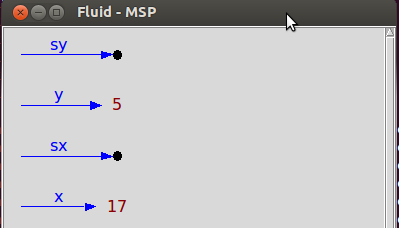
\includegraphics{fluid-1.png}

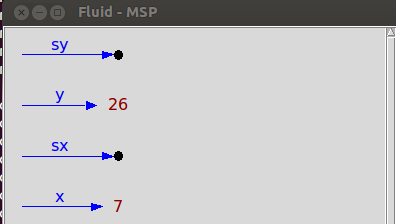
\includegraphics{fluid-2.png}

The source code of this assignment can be found on
\href{https://github.com/comco/concurrency-theory-assignments/tree/master/assignment-lecture-5.5}{GitHub}.
\end{document}
